%%% Please replace what is within each curly bracket with the correct information below. %%%
%%% The first field is already filled in for you.  %%%
\def\ClassName {CS188} % Your course 
\def\NameLast {Chen}  % Your last name
\def\NameFirst {Jianzhong}  % Your first name
\def\SID{23478230}  % Your SID
\def\Email{chenjianzhong@berkeley.edu} % Your pandagrader email
\def\Collaborators{None} % Any collaborators


%%%%% FILL IN YOUR ANSWERS TO EACH QUESTION SEE INSTRUCTIONS FOR EACH QUESTION.

\def\AnswerOneAi{
%%% Begin 1a(i) answer %%%%%%%%%%%%%%%%%%%%%%%%%%%%%%%%%%%%%%%%%%%%%%

%%% To cross out a value, use \cross. 
% For example, to cross out values 2,3, and 5 for variable V, do the following:
%                      V & 1 & \cross{2} & \cross{3} & 4 & \cross{5} & 6\\
P & \cross{1} & \cross{2} & \cross{3} & 4 & 5 & 6\\
B & \cross{1} & 2 & \cross{3} & 4 & \cross{5} & 6\\
C & 1 & 2 & 3 & 4 & 5 & 6\\
K & 1 & 2 & 3 & 4 & 5 & 6\\
I & \cross{1} & 2 & 3 & 4 & 5 & \cross{6}\\
M & \cross{1} & \cross{2} & \cross{3} & \cross{4} & 5 & 6\\


%%% End 1a(i) answer %%%%%%%%%%%%%%%%%%%%%%%%%%%%%%%%%%%%%%%%%%%%%%%%%
}
\def\AnswerOneAii{
%%% Begin 1a(ii) answer %%%%%%%%%%%%%%%%%%%%%%%%%%%%%%%%%%%%%%%%%%%%%%%%%

%%% For every bubble you want to fill, replace \mcqb with \mcqbubblefill.
%%% for example:              \mcqbubblefill {Answer} \hfill
\mcqb {P} \hfill 
\mcqb {B} \hfill 
\mcqb {C} \hfill 
\mcqb {K} \hfill
\mcqb {I} \hfill
\mcqbubblefill {M} \\

%%% End 1a(ii) answer  %%%%%%%%%%%%%%%%%%%%%%%%%%%%%%%%%%%%%%%%%%%%%%%%%
}
\def\AnswerOneAiii{
%%% Begin 1a(iii) answer %%%%%%%%%%%%%%%%%%%%%%%%%%%%%%%%%%%%%%%%%%%%%%%%%

%%% To cross out a value, use \cross. 
% For example, to cross out values 2,3, and 5 for variable V, do the following:
%                  V & 1 & \cross{2} & \cross{3} & 4 & \cross{5} & 6\\
P &   &   &   &  &   &  6\\
B & \cross{1} & \cross{2} & \cross{3} & 4 & \cross{5} & \cross{6}\\
C & 1 & 2 & 3 & 4 & 5 & \cross{6}\\
K & 1 & 2 & 3 & 4 & 5 & \cross{6}\\
I & \cross{1} & 2 & 3 & 4 & 5 & \cross{6}\\
M & \cross{1} & \cross{2} & \cross{3} & \cross{4} & 5 & \cross{6}\\

%%% End 1a(iii) answer  %%%%%%%%%%%%%%%%%%%%%%%%%%%%%%%%%%%%%%%%%%%%%%%%%%%
}
\def\AnswerOneAiv{
%%% Begin 1a(iv) answer %%%%%%%%%%%%%%%%%%%%%%%%%%%%%%%%%%%%%%%%%%%%%%%%%
Variable & \# violated\\
\hline
P& \solution{}{0}\\ %%% Replace ? with an integer within the brackets
\hline
B&\solution{}{0}\\ %%% Replace ? with an integer within the brackets
\hline
C&\solution{}{1}\\ %%% Replace ? with an integer within the brackets
\hline
K&\solution{}{0}\\ %%% Replace ? with an integer within the brackets
\hline
I&\solution{}{2}\\ %%% Replace ? with an integer within the brackets
\hline
M&\solution{}{0}\\ %%% Replace ? with an integer within the brackets
\hline
\end{tabular} \hspace{2cm}&
\begin{tabular}{|c|c|c|c|c|c|c|}
\hline
&1&2&3&4&5&6\\
\hline
% Example:
% V & x & x & x & x & x & x &  

P& & & & & &\\ %% put an "x" between the &'s to mark a cell.
\hline
B& & & & & &\\ %% put an "x" between the &'s to mark a cell.
\hline
C& & x & & & &\\ %% put an "x" between the &'s to mark a cell.
\hline
K& & & & & &\\ %% put an "x" between the &'s to mark a cell.
\hline
I& & x & x & & &\\ %% put an "x" between the &'s to mark a cell.
\hline
M& & & & & &\\ %% put an "x" between the &'s to mark a cell.
\hline
%%% End 1a(iv) answer %%%%%%%%%%%%%%%%%%%%%%%%%%%%%%%%%%%%%%%%%%%%%%%%%%%%
}

%%% Answers to 2a here. Put an x inside the curly brackets to mark, otherwise, leave blank.
\def\AnswerOneBi{

%%% Begin 1b(i) answer %%%%%%%%%%%%%%%%%%%%%%%%%%%%%%%%%%%%%%%%%%%%%%%%%%%%%
Algorithm 1 & Algorithm 2 & Algorithm 3\\
\hline
&&\\
% For example, to select the first column on a row:
% \sol{Answer 1} & {Answer 2} & {Answer 3}\\
{A-B-C-D-E-F} & {A-B-C-D-E-F} & \sol{A-B-C-D-E-F}\\ %% Put \sol in front of ordering to circle it.
&&\\
{F-E-D-C-B-A} & {F-E-D-C-B-A} & \sol{F-E-D-C-B-A}\\ %% Put \sol in front of ordering to circle it.
&&\\
{C-A-B-D-E-F} & \sol{C-A-B-D-E-F} & \sol{C-A-B-D-E-F}\\ %% Put \sol in front of ordering to circle it.
&&\\
{B-D-A-F-E-C} & {B-D-A-F-E-C} & \sol{B-D-A-F-E-C}\\ %% Put \sol in front of ordering to circle it.
&&\\
{D-E-F-C-B-A} & {D-E-F-C-B-A} & \sol{D-E-F-C-B-A}\\ %% Put \sol in front of ordering to circle it.
&&\\
{B-C-D-A-E-F} & \sol{B-C-D-A-E-F} & \sol{B-C-D-A-E-F}\\ %% Put \sol in front of ordering to circle it.

%%% End 1b(i) answer %%%%%%%%%%%%%%%%%%%%%%%%%%%%%%%%%%%%%%%%%%%%%%%%%%%%%
}
\def\AnswerOneBii{

%%% Begin 1b(ii) answer %%%%%%%%%%%%%%%%%%%%%%%%%%%%%%%%%%%%%%%%%%%%%%%%%%%
Algorithm 1 & Algorithm 2 & Algorithm 3\\
\hline
&&\\

% For example, to select the first column on a row:
% \sol{Answer 1} & {Answer 2} & {Answer 3}\\
{C-F-A-B-E-D-G-H} & {C-F-A-B-E-D-G-H} & \sol{C-F-A-B-E-D-G-H} \\ %% Put \sol in front of ordering to circle it.
&&\\
{F-C-A-H-E-B-D-G} & {F-C-A-H-E-B-D-G} & \sol{F-C-A-H-E-B-D-G} \\ %% Put \sol in front of ordering to circle it.
&&\\
{A-B-C-E-D-F-G-H} & {A-B-C-E-D-F-G-H} & {A-B-C-E-D-F-G-H} \\ %% Put \sol in front of ordering to circle it.
&&\\
{G-C-H-F-B-D-E-A} & {G-C-H-F-B-D-E-A} & \sol{G-C-H-F-B-D-E-A} \\ %% Put \sol in front of ordering to circle it.
&&\\
{A-B-E-D-G-H-C-F} & {A-B-E-D-G-H-C-F} & {A-B-E-D-G-H-C-F} \\ %% Put \sol in front of ordering to circle it.
&&\\
{A-D-B-G-E-H-C-F} & {A-D-B-G-E-H-C-F} & {A-D-B-G-E-H-C-F} \\ %% Put \sol in front of ordering to circle it.

%%% End 1b(ii) answer %%%%%%%%%%%%%%%%%%%%%%%%%%%%%%%%%%%%%%%%%%%%%%%%%%%
}

\def\AnswerOneCi {
%%% Begin Answer 1c(i) %%%%%%%%%%%%%%%%%%%%%%%%%%%%%%%%%%%%%%%%%%%%%%%%%%

%%% Replace \mcqb with \mcqbubblefill to select your answer(s).
& \mcqbubblefill Neither MRV nor LCV can have an effect.\\\\
& \mcqb Only MRV can have an effect.\\\\
& \mcqb Only LCV can have an effect .\\\\
& \mcqb Both MRV and LCV can have an effect.\\\\

%%% End Answer 1c(i) %%%%%%%%%%%%%%%%%%%%%%%%%%%%%%%%%%%%%%%%%%%%%%%%%%%%
}

\def\AnswerOneCii {
%%% Begin Answer 1c(i) %%%%%%%%%%%%%%%%%%%%%%%%%%%%%%%%%%%%%%%%%%%%%%%%%%

%%% %%% Begin Answer 1c(ii) %%%%%%%%%%%%%%%%%%%%%%%%%%%%%%%%%%%%%%%%%%%%%%%%%%

%%% Replace \mcqb with \mcqbubblefill to select your answer(s).
& \mcqb Neither MRV nor LCV can have an effect.\\\\
& \mcqbubblefill Only MRV can have an effect.\\\\
& \mcqb Only LCV can have an effect .\\\\
& \mcqb Both MRV and LCV can have an effect.\\\\
%%% End Answer 1c(ii) %%%%%%%%%%%%%%%%%%%%%%%%%%%%%%%%%%%%%%%%%%%%%%%%%%%%
}

\def\AnswerOneCiii {
%%% Begin Answer 1c(iii) %%%%%%%%%%%%%%%%%%%%%%%%%%%%%%%%%%%%%%%%%%%%%%%%%%

%%% Replace \mcqb with \mcqbubblefill to select your answer(s).
& \mcqb Neither MRV nor LCV can have an effect.\\\\
& \mcqbubblefill Only MRV can have an effect.\\\\
& \mcqb Only LCV can have an effect .\\\\
& \mcqb Both MRV and LCV can have an effect.\\\\
%%% End Answer 1c(iii) %%%%%%%%%%%%%%%%%%%%%%%%%%%%%%%%%%%%%%%%%%%%%%%%%%%%
}

\def\AnswerOneCiv {
%%% End Answer 1c(iv) %%%%%%%%%%%%%%%%%%%%%%%%%%%%%%%%%%%%%%%%%%%%%%%%%%%%

%%% Replace \mcqb with \mcqbubblefill to select your answer(s).
& \mcqb Neither MRV nor LCV can have an effect.\\\\
& \mcqbubblefill Only MRV can have an effect.\\\\
& \mcqb Only LCV can have an effect .\\\\
& \mcqb Both MRV and LCV can have an effect.\\\\
%%% End Answer 1c(iv) %%%%%%%%%%%%%%%%%%%%%%%%%%%%%%%%%%%%%%%%%%%%%%%%%%%%
}

\def\AnswerOneCv {
%%% End Answer 1c(v) %%%%%%%%%%%%%%%%%%%%%%%%%%%%%%%%%%%%%%%%%%%%%%%%%%%%

%%% Replace \mcqb with \mcqbubblefill to select your answer(s).
& \mcqb Neither MRV nor LCV can have an effect.\\\\
& \mcqbubblefill Only MRV can have an effect.\\\\
& \mcqb Only LCV can have an effect .\\\\
& \mcqb Both MRV and LCV can have an effect.\\\\
%%% End Answer 1c(v) %%%%%%%%%%%%%%%%%%%%%%%%%%%%%%%%%%%%%%%%%%%%%%%%%%%%
}

%%%%%%%%%%%%%%%%%%%%%% DO NOT CHANGE ANYTHING BELOW THIS LINE %%%%%%%%%%%%%%%%%%%%%%%%%
\def \showSolutions {} 

\documentclass[twoside]{article}
\usepackage{class}
\usepackage{graphicx}
\graphicspath{{./figs/}}
\usepackage{amsmath, amsthm, amssymb}
\usepackage{enumerate}
\usepackage{wrapfig}
\usepackage{color}
\usepackage{pifont}
\usepackage{mdwlist}
\usepackage[lofdepth,lotdepth]{subfig}
\usepackage{mdwlist}
\usepackage{wasysym}

\usepackage{ulem}
\title{Written HW2}

\usepackage{multirow}

\pagestyle{myheadings}

% Bubbles for multiple choice questions
\newcommand{\mcqbubble}{\bigcirc}
\newcommand{\mcqbubblefill}{\solution{\mcqb}{$\Large\newmoon$\ \ }}

% shorthand
\newcommand{\mcqb}{$\bigcirc$\ \ }
\newcommand{\mcqs}{\solution{\mcqb}{$\Large\newmoon$\ \ }}
\newcommand{\cross}[1]{{\color{blue}\sout{#1}}}
\newcommand{\sol}[1]{\solutioncircle{#1}}




\renewcommand{\P}{\mathbf{P}}
\newcommand{\eat}[1]{\ignorespaces}
\newcommand{\X}{\ding{110}}
\newcommand{\F}{$\bullet$}
\newcommand{\Pac}{$<$}
\def\truefalse{\vspace{0.3in} \item (\emph{true} or \emph{false}) }
\def\indep{\perp\!\!\!\perp}
\def\sgn{\mathop{\mathrm{sign}}}

\begin{document}
\thispagestyle{empty}
\maketitle


\smallskip
\smallskip
\textbf{INSTRUCTIONS}

\begin{itemize}
\item \textbf{Due:} Monday, February 10th, 2014 11:59 PM
\item \textbf{Policy:} Can be solved in groups (acknowledge collaborators) but must
be written up individually. However,
we strongly encourage you to first work alone for about 30 minutes total in order to simulate an exam environment.  Late homework
will not be accepted.
\item \textbf{Format:}  Submit the answer sheet pdf containing your answers. Page 1
must be this page, with your name,
SID, and pandagrader email filled in. Page 2 must contain your answers
to question 1 part a. Page 3 must contain your answers to question 1 part b. Page 4 must contain your answers to question 1 part c.
You should solve the questions on this handout (either through a pdf annotator, or by printing, then scanning; we recommend the latter to match exam setting). Alternatively, you can typeset a pdf on your own that has answers appearing in the same space (check edx/piazza for latex templating files and instructions).
\textbf{Make sure that your answers (typed or handwritten) are within the
dedicated regions for each question/part.  If you do not follow this format, we may deduct points.}

\item \textbf{How to submit:}  Go to www.pandagrader.com. Log in and click on the
class CS188 Spring 2014. Click
on the submission titled Written HW 2 and upload your pdf containing your answers. If this is your first time using
pandagrader, you will have to set your password before logging in the
first time.  To do so, click on "Forgot your password" on the login
page, and enter your email address on file with the registrar's office
(usually your @berkeley.edu email address). You will then receive an
email with a link to reset your password.

\end{itemize}


\begin{center}
\begin{tabular}{|r|c|}
\hline
\begin{minipage}{3cm}~\\Last Name~\\~\\\end{minipage} & \begin{minipage}[c][1cm][c]{8cm} ~ \NameLast \end{minipage}  \\
\hline
\begin{minipage}{3cm}~\\First Name~\\~\\\end{minipage} & \NameFirst \\
\hline
\begin{minipage}{3cm}~\\SID~\\~\\\end{minipage} & \SID \\
\hline
\begin{minipage}{3cm}~\\Email~\\~\\\end{minipage} & \Email \\
\hline
\begin{minipage}{3cm}~\\Collaborators~\\~\\\end{minipage} & \Collaborators \\
\hline

\end{tabular}
\end{center}



\vfill

\smallskip
\smallskip
\smallskip
\smallskip
\smallskip

\begin{center}
{\bf For staff use only}\\
\begin{Large}
\begin{tabular}{|r|r|}
\hline
Q. 1 Total\\
\hline

\qquad/30 \\
\hline
\end{tabular}\end{Large}
\end{center}

\begin{enumerate}


\q{30}{CSPs}
\begin{question}[]{\bf Pacman's new house}

After years of struggling through mazes, Pacman has finally made peace with the ghosts, Blinky, Pinky, Inky, and Clyde, and invited them to live with him and Ms. Pacman. The move has forced Pacman to change the rooming assignments in his house, which has 6 rooms. He has decided to figure out the new assignments with a CSP in which the variables are Pacman \textbf{(P)}, Ms. Pacman \textbf{(M)}, Blinky \textbf{(B)}, Pinky \textbf{(K)}, Inky \textbf{(I)}, and Clyde \textbf{(C)}, the values are which room they will stay in, from 1-6, and the constraints are:
\begin{table}[h]
\centering
\begin{tabular}{ll}
i) No two agents can stay in the same room&\\
ii) \textbf{P} $>$ 3 &
vi) \textbf{B} is even\\
iii) \textbf{K} is less than \textbf{P}&
vii) \textbf{I} is not 1 or 6\\
iv) \textbf{M} is either 5 or 6&
viii) $\vert$\textbf{I}-\textbf{C}$\vert$ = 1\\
v) \textbf{P} $>$ \textbf{M}&
ix) $\vert$\textbf{P}-\textbf{B}$\vert$ = 2
\end{tabular}
\end{table}
\begin{subquestion}[1]{\bf Unary constraints}
On the grid below cross out the values from each domain that are eliminated by enforcing unary constraints.
\solution{
\begin{table}[h]
\centering
\begin{tabular}{ccccccc}
P & 1 & 2 & 3 & 4 & 5 & 6\\
B & 1 & 2 & 3 & 4 & 5 & 6\\
C & 1 & 2 & 3 & 4 & 5 & 6\\
K & 1 & 2 & 3 & 4 & 5 & 6\\
I & 1 & 2 & 3 & 4 & 5 & 6\\
M & 1 & 2 & 3 & 4 & 5 & 6\\
\end{tabular}
\end{table}
}{
\begin{table}[h]
\centering
\begin{tabular}{ccccccc}
\AnswerOneAi
\end{tabular}
\end{table}
}
\end{subquestion}
\begin{subquestion}[1]{\bf MRV}
According to the Minimum Remaining Value (MRV) heuristic, which variable should be assigned to first?\\\\
\AnswerOneAii

\end{subquestion}

\begin{subquestion}[3]{\bf Forward Checking}
For the purposes of decoupling this problem from your solution to the
previous problem, assume we choose to assign P first, and assign it the value 6. What are the resulting domains after enforcing unary constraints (from part i) and running forward checking for this assignment?
\solution{
\begin{table}[h]
\centering
\begin{tabular}{ccccccc}
P &   &   &   &  &   &  6\\
B & 1 & 2 & 3 & 4 & 5 & 6\\
C & 1 & 2 & 3 & 4 & 5 & 6\\
K & 1 & 2 & 3 & 4 & 5 & 6\\
I & 1 & 2 & 3 & 4 & 5 & 6\\
M & 1 & 2 & 3 & 4 & 5 & 6\\

\end{tabular}
\end{table}
}{
\begin{table}[h]
\begin{center}
\begin{tabular}{ccccccc}
\AnswerOneAiii
\end{tabular}
\end{center}
\end{table}

}
\end{subquestion}

\begin{subquestion}[3]{\bf Iterative Improvement}
Instead of running backtracking search, you decide to start over and run
iterative improvement with the min-conflicts heuristic for value selection. Starting with the following assignment:\\\\
P:6, B:4, C:3, K:2, I:1, M:5\\\\
First, for each variable write down how many constraints it violates in the table below.\\
Then, in the table on the right, for all variables that could be selected for assignment, put an x in any box that corresponds to a possible value that could be assigned to that variable according to min-conflicts \textbf{in the next iteration}. When marking next values a variable could take on, only mark values different from the current one.

\begin{center}
\begin{tabular}{cc}
\begin{tabular}{|c|c|}
\hline
\AnswerOneAiv
\end{tabular}
\end{tabular}
\end{center}
\end{subquestion}

\end{question}
\newpage
\begin{question}[]{\bf Variable ordering}\\
We say that a variable X is backtracked if, after a value has been assigned to X, the recursion returns at X without a solution, and a different value must be assigned to X.\\
For this problem, consider the following three algorithms:
\begin{enumerate}
\item
Run backtracking search with no filtering
\item 
Initially enforce arc consistency, then run backtracking search with no filtering
\item
Initially enforce arc consistency, then run backtracking search while enforcing arc consistency after each assignment\\
\end{enumerate}

\begin{subquestion}[6]{}\\
For each algorithm, circle all orderings of variable assignments that guarantee that no backtracking will be necessary when finding a solution to the CSP represented by the following constraint graph.\\\\
\begin{table}[h]
\begin{tabular}{cc}
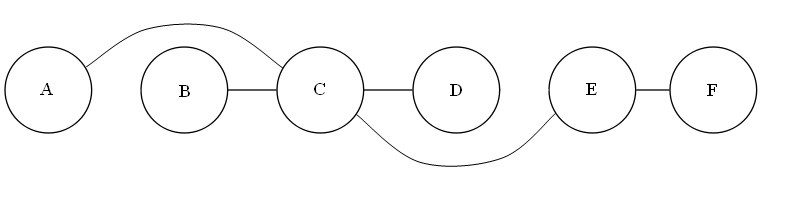
\includegraphics[scale=.4]{figures/tree.png}
&
\begin{tabular}{c|c|c}
\AnswerOneBi
\end{tabular}
\end{tabular}
\end{table}\\

\end{subquestion}
\begin{subquestion}[6]{}\\
For each algorithm, circle all orderings of variable assignments that guarantee that no more than two variables will be backtracked when finding a solution to the CSP represented by the following constraint graph.\\\\

\begin{table}[h]
\centering
\begin{tabular}{cc}
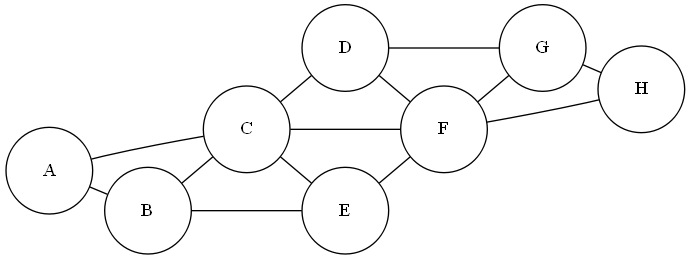
\includegraphics[scale=.3]{figures/csp_graph.png}
&
\begin{tabular}{c|c|c}
\AnswerOneBii
\end{tabular}
\end{tabular}
\end{table}
\end{subquestion}
\end{question}
\newpage
\begin{question}[]{\bf All Satisfying Assignments}
Now consider a modified CSP in which we wish to find every possible satisfying assignment, rather than just one such assignment as in normal CSPs. In order to solve this new problem, consider a new algorithm which is the same as the normal backtracking search algorithm, except that when it sees a solution, instead of returning it, the solution gets added to a list, and the algorithm backtracks. Once there are no variables remaining to backtrack on, the algorithm returns the list of solutions it has found.\\\\
For each graph below, select whether or not using the MRV and/or LCV heuristics could affect the number of leaf nodes in the search tree in this new situation.


\begin{subquestion}[2]{}\\
\begin{tabular}{cl}
\multirow{1}{*}{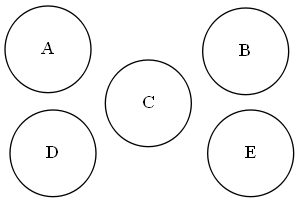
\includegraphics[scale=0.5]{figures/disconnected.png} \hspace{1.4in}}
\AnswerOneCi

\end{tabular}\\
\end{subquestion}

\vspace{-.1in}
\begin{subquestion}[2]{}\\
\begin{tabular}{cl}


\multirow{1}{*}{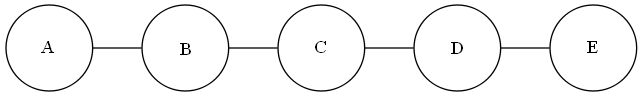
\includegraphics[scale=0.5]{figures/chain.png} \hspace{0.260in}}
\AnswerOneCii

\end{tabular}\\
\end{subquestion}
\vspace{-.19in}
\begin{subquestion}[2]{}\\
\begin{tabular}{cl}

\multirow{1}{*}{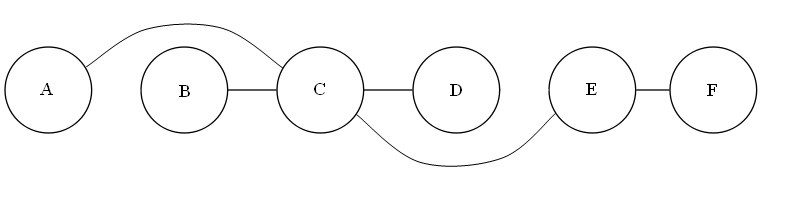
\includegraphics[width=3in]{figures/tree.png}}\\\\
\AnswerOneCiii

\end{tabular}
\end{subquestion}
\vspace{-.19in}
\begin{subquestion}[2]{}\\
\begin{tabular}{cl}

\multirow{1}{*}{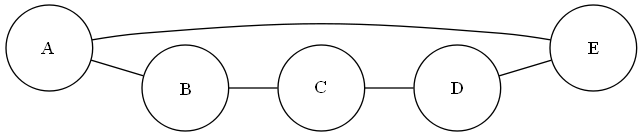
\includegraphics[width=3in]{figures/circle.png}} \\\\
\AnswerOneCiv

\end{tabular}
\end{subquestion}

\vspace{-.15in} 
\begin{subquestion}[2]{}\\
\begin{tabular}{cl}

\multirow{1}{*}{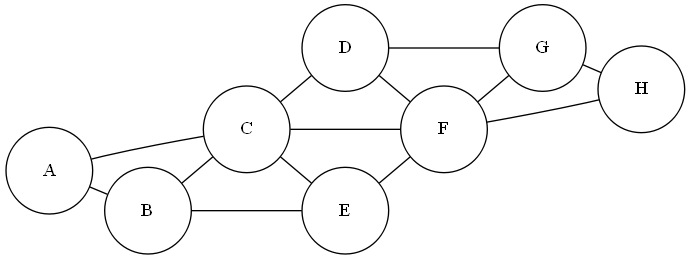
\includegraphics[width=3in]{figures/csp_graph.png}} \\\\
\AnswerOneCv

\end{tabular}
\end{subquestion}



\end{question}
\newpage
\end{enumerate}

\end{document}